%%%%%%%%%%%%%%%%%%%%%%%%%%%%%%%%%%%%%%%%%
% Beamer Presentation
% LaTeX Template
% Version 1.0 (10/11/12)
%
% This template has been downloaded from:
% http://www.LaTeXTemplates.com
%
% License:
% CC BY-NC-SA 3.0 (http://creativecommons.org/licenses/by-nc-sa/3.0/)
%
%%%%%%%%%%%%%%%%%%%%%%%%%%%%%%%%%%%%%%%%%

%----------------------------------------------------------------------------------------
%	PACKAGES AND THEMES
%----------------------------------------------------------------------------------------

\documentclass{beamer}

\mode<presentation> {

% The Beamer class comes with a number of default slide themes
% which change the colors and layouts of slides. Below this is a list
% of all the themes, uncomment each in turn to see what they look like.

%\usetheme{default}
%\usetheme{AnnArbor}
%\usetheme{Antibes}
%\usetheme{Bergen}
%\usetheme{Berkeley}
%\usetheme{Berlin}
%\usetheme{Boadilla}
%\usetheme{CambridgeUS}
%\usetheme{Copenhagen}
%\usetheme{Darmstadt}
%\usetheme{Dresden}
%\usetheme{Frankfurt}
%\usetheme{Goettingen}
%\usetheme{Hannover}
%\usetheme{Ilmenau}
%\usetheme{JuanLesPins}
%\usetheme{Luebeck}
%\usetheme{Madrid}
%\usetheme{Malmoe}
%\usetheme{Marburg}
%\usetheme{Montpellier}
%\usetheme{PaloAlto}
%\usetheme{Pittsburgh}
%\usetheme{Rochester}
%\usetheme{Singapore}
%\usetheme{Szeged}
\usetheme{Warsaw}
%\beamertemplatenavigationsymbolsempty

% As well as themes, the Beamer class has a number of color themes
% for any slide theme. Uncomment each of these in turn to see how it
% changes the colors of your current slide theme.

%\usecolortheme{albatross}
%\usecolortheme{beaver}
%\usecolortheme{beetle}
%\usecolortheme{crane}
%\usecolortheme{dolphin}
%\usecolortheme{dove}
%\usecolortheme{fly}
%\usecolortheme{lily}
%\usecolortheme{orchid}
%\usecolortheme{rose}
%\usecolortheme{seagull}
%\usecolortheme{seahorse}
%\usecolortheme{whale}
%\usecolortheme{wolverine}

%\setbeamertemplate{footline} % To remove the footer line in all slides uncomment this line
%\setbeamertemplate{footline}[page number] % To replace the footer line in all slides with a simple slide count uncomment this line

%\setbeamertemplate{navigation symbols}{} % To remove the navigation symbols from the bottom of all slides uncomment this line
}

\usepackage{graphicx} % Allows including images
\usepackage{booktabs} % Allows the use of \toprule, \midrule and \bottomrule in tables
\usepackage{etex}
\usepackage[T1]{fontenc}
\usepackage[utf8]{inputenc}
\usepackage[english]{babel}
\usepackage{cite}
\usepackage{amsmath,amsfonts,amssymb,amsthm}
\usepackage{mathrsfs,mathtools}
\usepackage{graphicx}
\usepackage{float}

\usepackage{hyperref} % References become hyperlinks.
\hypersetup{
	%colorlinks = true,
	linkcolor = {blue},
	urlcolor = {red},
	citecolor = {blue},
	%pdfenconing=auto,
}
\usepackage{wrapfig}
%\usepackage{arydshln}
\usepackage{array}
\usepackage[T1]{fontenc} 
\usepackage{bm}
\usepackage{multicol, multirow}
\usepackage{grffile,pgf,tikz}
\usepackage{verbatim}
\usepackage{graphicx}
\usepackage{animate}
\usepackage{caption}
\usepackage{subcaption}

% Default fixed font does not support bold face
\DeclareFixedFont{\ttb}{T1}{txtt}{bx}{n}{12} % for bold
\DeclareFixedFont{\ttm}{T1}{txtt}{m}{n}{12}  % for normal

% Custom colors
\usepackage{color}
\definecolor{deepblue}{rgb}{0,0,0.5}
\definecolor{deepred}{rgb}{0.6,0,0}
\definecolor{deepgreen}{rgb}{0,0.5,0}

\usepackage{listings}

% Python style for highlighting
\newcommand\pythonstyle{\lstset{
		language=Python,
		basicstyle=\ttm,
		morekeywords={self},              % Add keywords here
		keywordstyle=\ttb\color{deepblue},
		emph={MyClass,__init__},          % Custom highlighting
		emphstyle=\ttb\color{deepred},    % Custom highlighting style
		stringstyle=\color{deepgreen},
		frame=tb,                         % Any extra options here
		showstringspaces=false
}}


% Python environment
\lstnewenvironment{python}[1][]
{
	\pythonstyle
	\lstset{#1}
}
{}

% Python for external files
\newcommand\pythonexternal[2][]{{
		\pythonstyle
		\lstinputlisting[#1]{#2}}}

% Python for inline
\newcommand\pythoninline[1]{{\pythonstyle\lstinline!#1!}}



\usetikzlibrary{matrix}
\usetikzlibrary{shapes.geometric,calc,arrows}

%\usepackage{unicode-math}
%\setmathfont{XITS Math}
%\setmathfont[version=setB,StylisticSet=1]{XITS Math}


\theoremstyle{plain}
\newtheorem{teo}{Teorema}
%\newtheorem{lemma}[teo]{Lemma}
\newtheorem{prop}[teo]{Proposizione}
\newtheorem{post}{Postulato}
\newtheorem{cor}[teo]{Corollario}


\theoremstyle{definition}
\newtheorem{defn}{Definizione}
\newtheorem{exmp}[defn]{Esempio}
\newtheorem{oss}[defn]{Osservazione}
\newtheorem{prob}{Problema}
\newtheorem*{prob*}{Problema}
\newtheorem{hint}{Indizio}
\newtheorem*{notaz}{Notazione}

\theoremstyle{remark}
\newtheorem*{rem}{Remark}


\newcommand{\C}{\mathbb{C}}
\newcommand{\R}{\mathbb{R}}
\newcommand{\K}{\mathbb{K}}
\newcommand{\Q}{\mathbb{Q}}
\newcommand{\Z}{\mathbb{Z}}
\newcommand{\N}{\mathbb{N}}
\newcommand{\M}{\mathbb{M}}
\newcommand{\LL}{\mathscr{L}}
\newcommand{\HH}{\mathbb{H}}
\newcommand{\SP}{\mathbb{S}}
\newcommand{\dsum}{\displaystyle\sum}
\newcommand{\dint}{\displaystyle\int}
\newcommand{\scal}[2]{\langle #1,#2 \rangle}
\newcommand{\norm}[1]{\lVert#1\rVert}
\newcommand{\eval}[3]{\Big[ #1 \Big]_{#2}^{#3}}
%\newcommand{\sob}[3]{W^{#1, #2}(#3)}
%\newcommand{\sobzero}[3]{W_{0}^{#1, #2}(#3)}
%\newcommand{\sobloc}[3]{W_{\text{loc}}^{#1, #2}(#3)}
\newcommand{\weakconv}{\rightharpoonup}
\newcommand{\weakconvs}{\overset{\ast}{\rightharpoonup}}
\newcommand{\prox}{\text{prox}}


\newcommand{\dx}{\text{d}x}
\newcommand{\dt}{\text{d}t}
\newcommand{\dy}{\text{d}y}
\newcommand{\diff}{\text{d}}
\newcommand{\dX}{\text{d}\bm{x}}
\newcommand{\dFX}{\text{d}F(\bm{x})}
\newcommand{\dfX}{\text{d}f(\bm{x})}
\newcommand{\dFx}{\text{d}F(x)}
\newcommand{\dfx}{\text{d}f(x)}
\newcommand{\X}{\bm{X}}
\newcommand{\x}{\bm{x}}
\newcommand{\B}{\bm{b}}
\newcommand{\F}{\mathcal{F}}
\newcommand{\Pro}{\mathbf{P}}
\newcommand{\E}{\mathbb{E}}
\newcommand{\bh}{\hat{\bm{b}}}
\newcommand{\Sh}{\hat{S}}
\newcommand{\dmu}{\text{d}\mu(\B)}
\newcommand{\Ph}{\hat{\mathbf{P}}}
\newcommand{\Ct}{\tilde{C}}
\newcommand{\Dt}{\tilde{D}}


\DeclareMathOperator{\tr}{tr}
\DeclareMathOperator{\Hom}{Hom}
\DeclareMathOperator{\End}{End}
\DeclareMathOperator{\Orb}{Orb}
\DeclareMathOperator{\Stab}{Stab}
\DeclareMathOperator{\Fix}{Fix}
\DeclareMathOperator{\Ind}{Ind}
\DeclareMathOperator{\Ker}{Ker}
\DeclareMathOperator{\Imm}{Im}
\DeclareMathOperator{\supp}{supp}
\DeclareMathOperator{\Res}{Res}
\DeclareMathOperator{\Id}{Id}
\DeclareMathOperator{\Char}{char}
\DeclareMathOperator{\cof}{cof}
\DeclareMathOperator{\rk}{rk}
\DeclareMathOperator{\dist}{dist}
\DeclareMathOperator{\dive}{div}
\DeclareMathOperator{\Span}{Span}
\DeclareMathOperator{\Lip}{Lip}
\DeclareMathOperator{\diam}{diam}
\DeclareMathOperator{\Int}{int}
\DeclareMathOperator{\extr}{extr}
\DeclareMathOperator{\conv}{conv}
\DeclareMathOperator{\divergence}{div}
\DeclareMathOperator{\baric}{bar}
\DeclareMathOperator*{\argmax}{arg\,max}
\DeclareMathOperator*{\argmin}{arg\,min}

\newcommand{\grad}{\nabla}
\newcommand{\perim}{\mathcal{P}}%%%%%%%%%%%%%%%
%%ATTENZIONE: HO TOLTO LE PARENTESI, ORA \perim METTE SOLO LA P
\newcommand{\symmdiff}{\Delta}
\newcommand{\bdry}{\partial}
\newcommand{\clos}[1]{\overline{#1}}
\newcommand{\lebesgue}{\ensuremath{\mathscr{L}}}


%definizioni che servono solo per la tesi magistrale
\newcommand{\FF}{\mathcal{F}}	%funzionale completo dell'energia
\newcommand{\FFF}{\widetilde{\mathcal{F}}} %funzionale dell'energia sui sottoinsiemi disgiunti
\newcommand{\GG}{\mathcal{G}}	%funzionale con potenza positiva al posto del perimetro
\newcommand{\RR}{\mathcal{R}}	%funzionale di Riesz
\newcommand{\riesz}[1]{\iint_{#1 \times #1}\frac{1}{|x-y|^{N-\alpha}}\dx\dy}
\newcommand{\genriesz}[2]{\iint_{#1 \times #1}#2(|x-y|)\dx\dy}



%debug
\newcommand{\avviso}[1]{{\textcolor{red}{\textbf{#1}}}}


\newcommand\restr[2]{\ensuremath{\left.#1\right|_{#2}}}


\newcommand{\boh}{\textcolor{red}{\Huge\textbf{???}}}
\newcommand{\attenzione}{\textcolor{red}{\Huge\textbf{!!!}}}
\newcommand{\vitali}{\textcolor{red}{\Huge\textbf{Vitali}}}




%----------------------------------------------------------------------------------------
%	TITLE PAGE
%----------------------------------------------------------------------------------------

\title[Anomaly Detection with Robust Deep Autoencoders]{Anomaly Detection with Robust Deep Autoencoders} % The short title appears at the bottom of every slide, the full title is only on the title page
\subtitle[]{original article by C. Zhou and R. C. Peffenroth}
\author[Alessandro Trenta]{\emph{Alessandro Trenta}} % Your name
\institute[SNS] % Your institution as it will appear on the bottom of every slide, may be shorthand to save space
{Scuola Normale Superiore \\ % Your institution for the title page
% Your email address
}
\date{} % Date, can be changed to a custom date

\begin{document}

\begin{frame}
	\titlepage % Print the title page as the first slide
\end{frame}

\begin{frame}
	\tableofcontents
\end{frame}

\nocite{RAE}

\section{Background}

\begin{frame}
	\frametitle{Deep Autoencoders}
	\begin{itemize}
		\item A Deep Autoencoder (DAE) is constituted by two main components: an encoder $E$ and a Decoder $D$.
		\item The main objective of a DAE is to learn the identity map so that the reconstruction $\bar{X}=D(E(X))$ is as close as possible to the original input $X$.
		\item The encoder and decoder functions $E, D$ can be any kind of mapping between the data space and the coded space. Usually they are Deep Neural Networks e.g. FCNN complex models such as Long Short Term Memory (LSTM) or Gated Recurrent Units (GRU).
		\item The objective is usually to find the minimum reconstruction error w.r.t. some parametrized encoding and decoding functions and a distance (in this case the $L_2$ norm)
			\begin{equation}
				\min_{\theta, \phi}{\norm{X-D_{\theta}(E_{\phi}(X))}_{2}}
			\end{equation}
	\end{itemize}
\end{frame}

\begin{frame}
	\frametitle{Principal Component Analysis}
	\begin{itemize}
		\item Assume to have a set of $N$ samples of $n$ dimensional data, so that $X\in \R^{N\times n}$ s.t. each column has $0$ mean (we can just shift the data to fulfill this request).
		\item Principal Component Analysis (PCA) is defined as an orthogonal linear transformation such that the new coordinate system of $\R^{n}$ satisfies: 
			the $i$-th component of the coordinate system has the $i$-th greatest data variance if we project all samples on that component.
		\item Ideally we are trying to fit a $n$-ellipsoid into the data. The length of an axis of the ellipsoid represents the variance of data along that axis.
		\item PCA is often used for dimensionality reduction or encoding: we can project the data on the first $k<n$ principal components.
	\end{itemize}
\end{frame}

\begin{frame}
	\frametitle{Principal Component Analysis}
	Mathematically we can define:
		\begin{equation}
			w_1 = \argmax_{\norm{w}_{2}=1}{\norm{Xw}_{2}^2} = \argmax_{w}{\frac{w^TX^TXw}{w^Tw}}
		\end{equation}
		for the first component. Then for the $k$-th component we first subtract the first $k-1$ principal component from $X$
		\begin{equation}
			\hat{X}_{k} = X - \sum_{i=1}^{k-1}{Xw_{i}w_{i}^T}
		\end{equation}
		and finally solving again the similar problem:
		\begin{equation}
			w_k = \argmax_{\norm{w}_{2}=1}{\norm{\hat{X}_{k}w}_{2}^2} = \argmax_{w}{\frac{w^T\hat{X}_{k}^T\hat{X}_{k}w}{w^Tw}}
		\end{equation}
\end{frame}

\begin{frame}
	\frametitle{Robust Principal Component Analysis}
	\begin{itemize}
		\item Robust Principal Component Analysis (RPCA) is a generalization of PCA that aims to reduce the sensitivity of PCA to outliers.
		\item The idea is to find a low-dimensional representation of data cleaned from the sparse outliers that can disturb the PCA process.
		\item We therefore assume that data $X$ can be represented as $X = L + S$: $L$ has low rank and is the low-dimensional representation of $X$ while $S$ is a sparse matrix 
			consisting of the outlier elements that cannot be captured by the representation.
	\end{itemize}
\end{frame}

\begin{frame}
	\frametitle{Robust Principal Component Analysis}
	\begin{itemize}
		\item The problem can be addressed as:
			\begin{align}
				\min_{L,S}{\rho(L)+\lambda \norm{S}_{0}}\\
				\text{s. t. }\norm{X - L - S}_{F}^2=0 
			\end{align}
			where $\rho(\cdot)$ is the rank of a matrix and we used the zero norm.
		\item This optimization problem is NP-hard and tractable only for small metrices.
		\item Usually it is substituted by the following problem, which is convex and tractable also for large matrices:
			\begin{align}
				\min_{L,S}{\norm{L}_{*}+\lambda \norm{S}_{1}}\\
				\text{s. t. }\norm{X - L - S}_F^2=0
			\end{align}
			where $\norm{\cdot}_*$ is the nuclear norm i. e. the sum of singular values of a matrix.
	\end{itemize}
\end{frame}

\section{Robust Deep Autoencoders}

\begin{frame}
	\frametitle{Robust Deep Autoencoders}
	\begin{itemize}
		\item The main idea behind Robust Deep Autoencoders (RDAE) is to combine the representation learning of DAEs and the anomaly detection capability of RPCA.
		\item Noise and outliers are incompressible in the lower dimensional space we want to represent our data in.
		\item The objective is to learn a good low dimensional representation except for few exceptions.
		\item We will see two RDAE typed, one for $l_1$ regularization and one for $l_{2,1}$.
	\end{itemize}
\end{frame}

\begin{frame}
	\frametitle{RDAE with $l_1$ regularization}
	\begin{itemize}
		\item The RDAE objective is to decompose data $X=L_D+S$ just as in RPCA.
		\item By removing the noise $S$ the autoencoder can better reconstruct $L_D$.
		\item As before, the best choice to obtain a sparse $S$ would be to use a loss of the type $\norm{S}_0$ which counts the non-zero entries, solving the problem
			\begin{align}
				\min_{\theta}{\norm{L_D -D_{\theta}(E_{\theta}(L_D))}_2 + \lambda\norm{S}_0}\\
				\text{s.t. }X-L_D-S=0  
			\end{align}
		\item The parameter $\lambda$ controls the sparsity of $S$ and plays an essential role.
	\end{itemize}
\end{frame}

\begin{frame}
	\frametitle{The role of $\lambda$}
	\begin{itemize}
		\item As we said, the role of $\lambda$ is very important.
		\item A smaller $\lambda$ means that the norm of $S$ plays a less important role and much of the loss will come from the DAE.
		\item The model will reconstruct better but recognize less outliers. This could be helpful if we want a more faithful representation e.g. for supervised tasks.
		\item A larger $\lambda$, instead, gives more importance to the norm of $S$ as a loss.
		\item This means that the model will recognize more (or even too much) outliers, sacrificing some reconstruction performance.
	\end{itemize}
\end{frame}

	
\begin{frame}
	\frametitle{The true objective}
	\begin{itemize}
		\item As for the RPCA the previous loss is non tractable. We then instead focus on the following problem:
			\begin{align}
				\min_{\theta}{\norm{L_D -D_{\theta}(E_{\theta}(L_D))}_2 + \lambda\norm{S}_1}\\
				\text{s.t. }X-L_D-S=0  
			\end{align}
			Notice two things:
		\item The autoencoder is trained with $L_D$, the part of its decomposition assumed to be outliers and noise free.
		\item There is no specific requirement about the DAE, in fact $D_{\theta}$ and $E_{\theta}$ are generic decoder, encoder functions.
	\end{itemize}
\end{frame}

\begin{frame}
	\frametitle{RDAE with $l_{2,1}$ regularization}
	\begin{itemize}
		\item The RDAE with $l_1$ penalization assumes that outliers and noise are not structured. The $l_1$ penalty is indeed just a regularization to induce sparsity.
		\item In general we can have multiple types of errors: an instrument that corrupts an input feature or outliers where the input data is in some way structurally different from normal data.
	\end{itemize}
\end{frame}

\begin{frame}
	\centering
	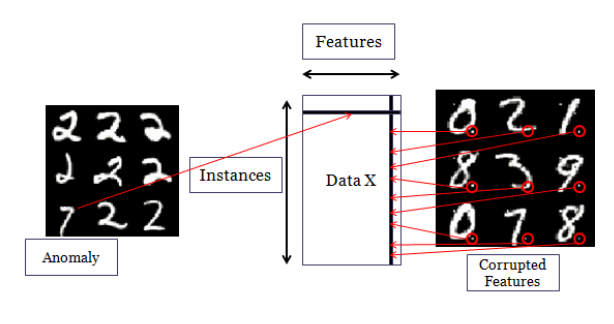
\includegraphics[width=0.9\linewidth]{Images/diff_anomalies.png}
\end{frame}

\begin{frame}
	\frametitle{The $l_{2,1}$ norm}
	\begin{itemize}
		\item The $l_{2,1}$ norm is defined as ($X\in \R^{N\times n}$):
			\begin{equation}
				\norm{X}_{2,1} = \sum_{j=1}^{n}{\norm{X_j}_{2}} = \sum_{j=1}^{n}{\left(\sum_{i=1}^{N}|X_{ij}|^{2}\right)^{\frac{1}{2}}}
			\end{equation}
		\item The $l_{2,1}$ norm can be seen as introducting a $l_2$ norm regularization over each feature and then adding a $l_1$ regularization accross features.
		\item We can also do the other way around: to recognize data anomalies (by row) just apply the $l_{2,1}$ norm to $X^T$.
	\end{itemize}
\end{frame}

\begin{frame}
	\begin{itemize}
		\item The final optimization problem for the RDAE with $l_{2,1}$ regularization for data anomalies is then
			\begin{align}
				\min_{\theta}{\norm{L_D -D_{\theta}(E_{\theta}(L_D))}_2 + \lambda\norm{S^T}_{2,1}}\\
				\text{s.t. }X-L_D-S=0  
			\end{align}
		\item For detecting feature anomalies we just need to change the objective to
			\begin{align}
				\min_{\theta}{\norm{L_D -D_{\theta}(E_{\theta}(L_D))}_2 + \lambda\norm{S}_{2,1}}\\
				\text{s.t. }X-L_D-S=0  
			\end{align}
	\end{itemize}
\end{frame}

\section{RDAE training}

\begin{frame}
	\frametitle{The proximal operator}
	\begin{itemize}
		\item To see in detail the training procedure for the RDAE we first need to consider the proximal operator.
		\item For general optimization problems of the form $\min f(x)+\lambda g(x)$ where $g$ is convex some of the most used methods require to find
			\begin{equation}
				\prox_{\lambda, g}(x) = \argmin_{y}{g(y)+\frac{1}{2\lambda}\norm{x-y}_{2}^{2}}
			\end{equation}
		\item In this case we then want to obtain a solution of the problems
			\begin{align}
				\prox_{\lambda, l_1}(x) = \argmin_{y}{l_1(y)+\frac{1}{2\lambda}\norm{x-y}_{2}^{2}}\\
				\prox_{\lambda, l_{2,1}}(x) = \argmin_{y}{l_{2,1}(y)+\frac{1}{2\lambda}\norm{x-y}_{2}^{2}}
			\end{align}
	\end{itemize}
\end{frame}

\begin{frame}
	\begin{itemize}
		\item For the $l_1$ norm, the solution to the proximal problem is
			\begin{equation}
				\prox_{\lambda, l_1}(x) = \begin{cases}
					x_i - \lambda, & x_i>\lambda\\
					x_i + \lambda, & x_i<-\lambda\\
					0, & x_i\in[-\lambda, \lambda]
				\end{cases}
			\end{equation}
			which in the case of $S\in\R^{N\times n}$ gets applied element by element.
		\item For the $l_{2,1}$ norm, we obtain (let $S_{\cdot j}$ be the column vector $S_{ij}, j=1, \ldots, N$)
			\begin{equation}
				(\prox_{\lambda, l_{2,1}}(S))_{ij} = \begin{cases}
					S_{ij}-S_{ij} - \lambda\frac{S_{ij}}{\norm{S_{\cdot j}}_{2}}, & \norm{S_{\cdot j}}_{2} > \lambda\\
					0, & \norm{S_{\cdot j}}_{2} \leq \lambda
				\end{cases}
			\end{equation}
			if we are considering feature wise anomalies, substitute $S$ with $S^T$ for data anomalies.
	\end{itemize}
\end{frame}

\begin{frame}
	\frametitle{The main algorithm}
	\begin{itemize}
		\item The method used to train the RDAE is the Alternating Direction Method of Multipliers (ADMM).
		\item The main idea is to optimize the problem
			\begin{align}
				\min_{\theta}{\norm{L_D -D_{\theta}(E_{\theta}(L_D))}_2 + \lambda\norm{S^T}_{2,1}}\\
				\text{s.t. }X-L_D-S=0  
			\end{align}
			by doing it in two steps at each iteration.
		\item First, we fix $S$ and optimize the DAE loss $\norm{L_D -D_{\theta}(E_{\theta}(L_D))}_2$ with backpropagation as usual.
		\item Then, we fix $L_D$ and optimize the regularization term with the proximal method.
	\end{itemize}
\end{frame}

\begin{frame}
	The full procedure is the following: given input $X\in \R^{N\times n}$, initialize $L_D\in \R^{N\times n}, S\in \R^{N\times n}$ as zero matrices, 
	$L_S = X$ and initialize the DAE randomly. For each iteration do:
	\begin{itemize}
		\item $L_D = X - S$
		\item Minimize $\norm{L_D -D_{\theta}(E_{\theta}(L_D))}_2$ with backpropagation.
		\item Set $L_D = D(E(L_D))$ as the reconstruction.
		\item Set $S = X - L_D$.
		\item Optimize $S$ using a $\prox_{\lambda, l_{\cdot}}$ function of choice.
		\item If $c_1 = \frac{\norm{X-L_D-S}_2}{\norm{X}_2} < \epsilon$ or $c_2 = \frac{\norm{LS-L_D-S}_2}{\norm{X}_2} < \epsilon$ we have early convergence.
		\item Set $L_S = L_D + S$.
	\end{itemize}
	Return $L_D$ and $S$.
\end{frame}

\section{Results}

\begin{frame}
	\frametitle{Results}
	\begin{itemize}
		\item I tried to reproduce some of the results by the original article.
		\item For the main article results the database used was the MNIST digits database.
		\item The train data contains $50000$ samples while the test set contins $10000$ images.
		\item Data was flattened from images of shape $(28,28,1)$ into vectors of length $784$. Train data is then a matrix in $\R^{50000\times 784}$.
		\item Pixel walues are converted from integers between $0$ and $255$ to floats between $0$ and $1$.
	\end{itemize}
\end{frame}

\begin{frame}
	\frametitle{Implementation}
	\begin{itemize}
		\item The RDAE and the standard DAEs used in this experimental tries were implemented using Tensorflow $2.9.1$ on python $3.8$.
		\item For the random forest classifier and the isolation forest models were taken from SciKit-learn version $1.1.1$.
		\item Full implementation and details can be found on \hyperref{https://github.com/AlexThirty/SaMLMfTSA}{}{}{GitHub}
	\end{itemize}
\end{frame}

\begin{frame}
	\frametitle{$l_1$ Robust Deep Autoencoder}
	\begin{itemize}
		\item To assess the performance of the $l_1$ RDAE the proposed procedure is the following:
		\item The training images get corrupted with a percentage of pixel (from $5\%$ to $50\%$) changed to a random value between $0$ and $1$.
		\item Both the RDAE with $l_1$ regularization and a standard DAE (with same architecture as the DAE from the RDAE) are trained on these corrupted images.
		\item A random forest classifier is then trained on the feature extracted at the bottomneck layers of the two models.
		\item We test how these RF classifiers perform on the test set.
	\end{itemize}
\end{frame}

\begin{frame}
	\begin{itemize}
		\item This let us see how well the model is able to extract the important features of the images in a meaningful way.
		\item In this case the RDAE and DAE need to denoise the images and recognize which charactheristics are improtant.
		\item Both architectures are simple FCNN with layers of size $784$ (input), $200$ and $10$ (the bottleneck and hidden feature layer).
		\item The RDAE was trained for $10$ outer iterations with $50$ inner iterations each, while the DAE was trained for $100$ epochs. The batch size is $256$.
	\end{itemize}
\end{frame}

\begin{frame}
	\frametitle{$L_1$ RDAE analysis}
	\begin{itemize}
		\item Unfortunately, I could not replicate the results by the article.
		\item I tried with different values for the parameters and different setups.
		\item In any case, the $L_1$ RDAE performance was really similar to the performance of a simple Deep Autoencoder, in some cases worse.
		\item This is not to say that the RDAE has a poor performance, as we will see it can have some better reconstructions with corrupted data.
		\item The simpler approach seems to work better for supervised task with the hidden layer.
		\item The article was written when Tensorflow and other libraries were still in progress. It could also be that recent improvements benefit the DAE performance.
	\end{itemize}
\end{frame}

\begin{frame}
	\frametitle{Original results}
	\begin{figure}
		\centering
		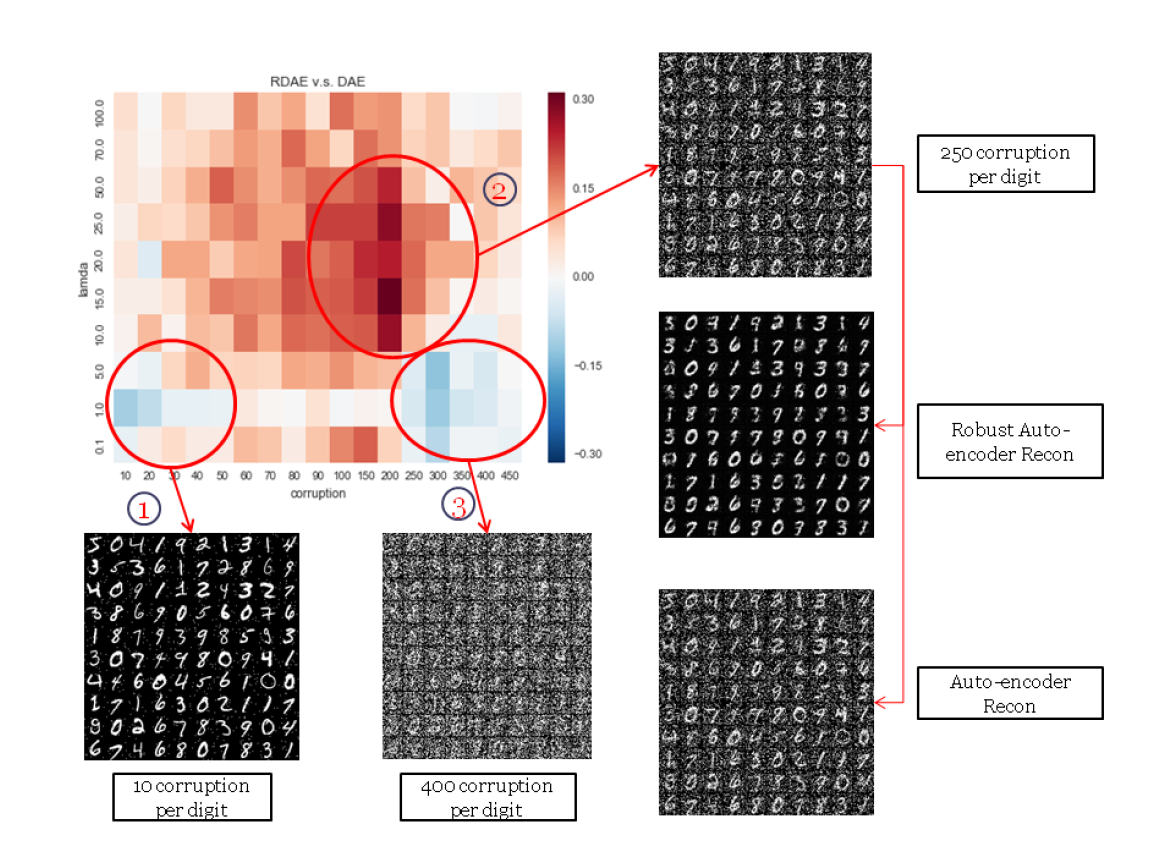
\includegraphics[width=0.8\linewidth]{Images/original_l1.png}
	\end{figure}
\end{frame}

\begin{frame}
	\frametitle{Deep Autoencoder RF performance}
	\begin{figure}
		\centering
		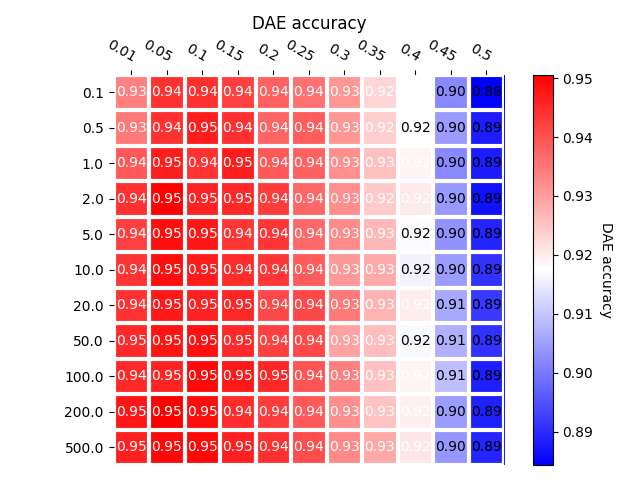
\includegraphics[width=0.7\linewidth]{Images/DAE_acc.png}
		\caption[]{Performance of the Random forest on the hidden layer of base Deep Autoencoder on different $\lambda$, corruption}
	\end{figure}
\end{frame}

\begin{frame}
	\frametitle{$l_1$ RDAE RF performance}
	\begin{figure}
		\centering
		
\includegraphics[width=0.7\linewidth]{Images/RAE_acc.png}
		\caption[]{Performance of the Random forest on the hidden layer of base $l_1$ RDAE on different $\lambda$, corruption}
	\end{figure}
\end{frame}

\begin{frame}
	\frametitle{Performance comparison}
	\begin{figure}
		\centering
		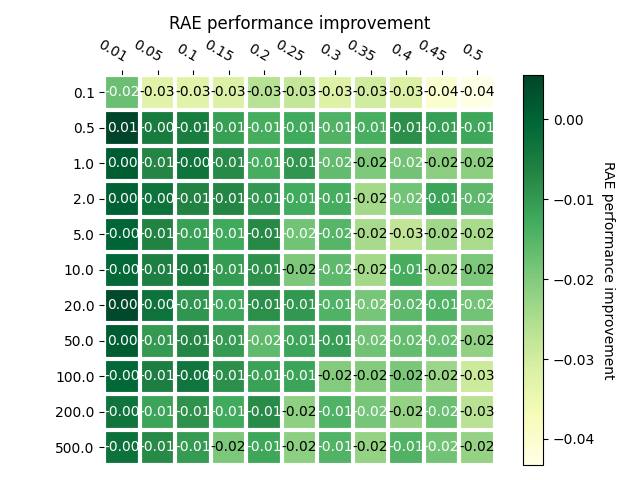
\includegraphics[width=0.7\linewidth]{Images/performance.png}
		\caption[]{Performance increase of using RDAE on different $\lambda$, corruption}
	\end{figure}
\end{frame}

\begin{frame}
	\frametitle{Comments on performance}
	\begin{itemize}
		\item As we can see the RDAE performed worse in each case.
		\item In general, the problem is not the RDAE which is not performing good enough.
		\item It seems indeed that the basic DAE performs really good, even on highly corrupted data.
	\end{itemize}
\end{frame}


\begin{frame}
	\frametitle{$l_{2,1}$ Robust Deep Autoencoder}
	\begin{itemize}
		\item The anomaly detection experiment is based on the recognizing of a specific digit of the MNIST dataset.
		\item First all the $4$ digit images in the training set are collected in our dataset.
		\item Then, some images are chose at random from all the other digits until they are around $5\%$ of total images in the dataset.
		\item This will be considered as the outliers of our data.
	\end{itemize}
\end{frame}


\begin{frame}
	\begin{itemize}
		\item The $l_{2,1}$ RDAE is trained on this dataset without any side information.
		\item Without telling the model which images are $4$ digits and which are outliers the model itself must recognize the latters from original data on his own.
		\item The model architecture is the same as for the $l_1$ RDAE experiment.
		\item The only parameter that requires tuning is $\lambda$.
	\end{itemize}
\end{frame}

\begin{frame}
	\begin{itemize}
		\item Model performance is assessed by seeing how it is able to recognize the correct "outliers".
		\item The metrics used are the accuracy, the precision score, the recall score and the F1 score defined down below.
			\begin{align}
				ACC = \frac{TP+TN}{P+N}\;\;\; P = \frac{TP}{TP+FP}\\
				R = \frac{TP}{TP+FN} \;\;\; F1 = 2\frac{P\cdot R}{P+R}
			\end{align}
		\item The F1 score, which tries to average in some way precision and recall, is the metrics used to select the $\lambda$ parameter.
		\item $\lambda$ is the only parameter that is fine tuned (in a semi-supervised way).
	\end{itemize}
\end{frame}

\begin{frame}
	\frametitle{Original performance}
	\begin{figure}
		\centering
		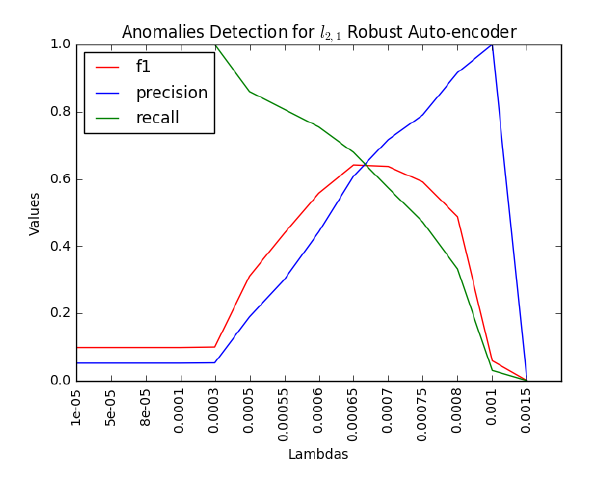
\includegraphics[width=0.7\linewidth]{Images/l21_perf_article.png}
		\caption[]{$L_{2,1}$ RDAE anomaly detection performance from original article}
	\end{figure}
\end{frame}

\begin{frame}
	\frametitle{Anomaly detection performance}
	\begin{figure}
		\centering
		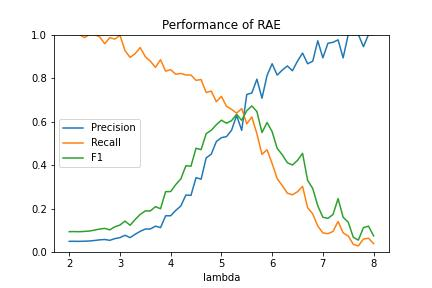
\includegraphics[width=0.8\linewidth]{Images/l21_experiment_from_0.1_to_10.1.jpg}
		\caption[]{$L_{2,1}$ RDAE anomaly detection performance. $\lambda$ from $2$ to $8$}
	\end{figure}
\end{frame}

\begin{frame}
	\frametitle{Anomaly detection performance}
	\begin{figure}
		\centering
		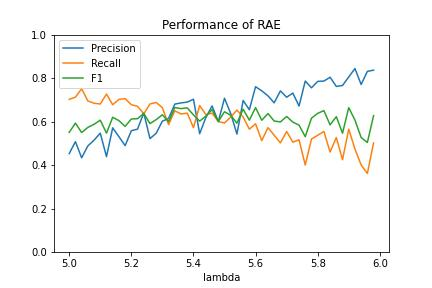
\includegraphics[width=0.8\linewidth]{Images/l21_experiment_from_5.0_to_6.0.jpg}
		\caption[]{$L_{2,1}$ RDAE anomaly detection performance. $\lambda$ from $5$ to $6$}
	\end{figure}
\end{frame}

\begin{frame}
	\frametitle{Anomaly detection performance}
	\begin{figure}
		\centering
		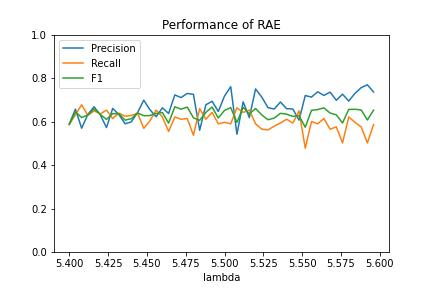
\includegraphics[width=0.8\linewidth]{Images/l21_experiment_from_5.4_to_5.6.jpg}
		\caption[]{$L_{2,1}$ RDAE anomaly detection performance. $\lambda$ from $5.4$ to $5.6$}
	\end{figure}
\end{frame}



\begin{frame}
	\begin{itemize}
		\item The maximum performance is obtained with $\lambda=5.468$ with an $F_1$ score of $0.668$.
		\item Focusing on all values from $\lambda=5$ to $\lambda=6$ the RDAE has an accuracy of over $95\%$ in recognizing anomalies. The $F_1$ score in this range is almost everytime above $0.55$.
		\item The $F_1$ score is almost everytime above $0.6$ for $\lambda$ in the $[5.4, 5.6]$ range.
		\item Best result obtained by the authors is an $F_1$ score of $0.64$ for $\lambda=0.00065$. This different value of $\lambda$ is in my opinion due to the different parameters of the neural network.
	\end{itemize}
\end{frame}


\begin{frame}
	\begin{itemize}
		\item We are now going to have a look at the final and reconstructed images obtained from the RDAE.
		\item For each value of $\lambda$ we have $3$ main images to look at: the reconstructionof the original images from the DAE in the RDAE, the final $L_D$ image (the "clean" version, in this case it should only contain $4$s) and the $S$ image, which should be non empty only for outliers.
		\item We look $3$ different values for $\lambda$: the best one identified above, $8.0$ which adds too much penalization with few outliers identified and $4.0$ which is a low value and a lot of $4$s are considered outliers.
	\end{itemize}
\end{frame}

\begin{frame}
	\frametitle{Original Images data}
	\begin{figure}
		\centering
		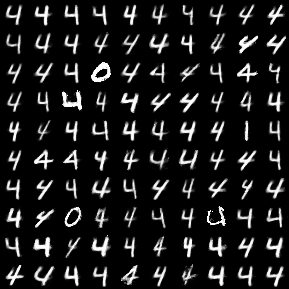
\includegraphics[width=0.5\linewidth]{Images/original_l21.png}
		\caption[]{Original images for the $L_{2,1}$ RDAE}
	\end{figure}
\end{frame}


\begin{frame}
	\frametitle{$\lambda=5.468$}
	\begin{figure}
		\centering
		\begin{subfigure}[b]{0.3\textwidth}
			\centering
			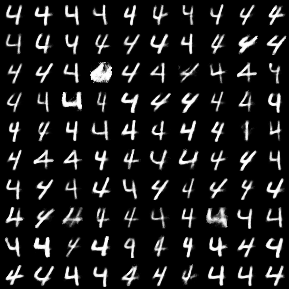
\includegraphics[width=\textwidth]{Images/l21R_5.468.png}
			\caption{Reconstruction}
		\end{subfigure}
		\hfill
		\begin{subfigure}[b]{0.3\textwidth}
			\centering
			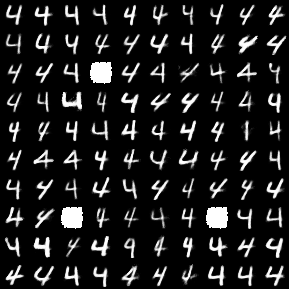
\includegraphics[width=\textwidth]{Images/l21L_5.468.png}
			\caption{Cleaned data}
		\end{subfigure}
		\hfill
		\begin{subfigure}[b]{0.3\textwidth}
			\centering
			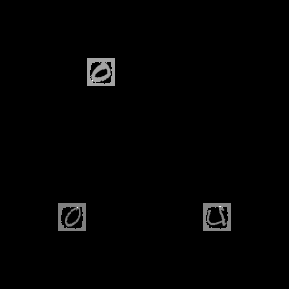
\includegraphics[width=\textwidth]{Images/l21S_5.468.png}
			\caption{Outliers detection}
		\end{subfigure}
		   \caption{Accuracy: $0.970$, precision: $0.722$, recall: $0.621$, F1 score: $0.668$}
   \end{figure}
\end{frame}

\begin{frame}
	\frametitle{$\lambda=8.0$}
	\begin{figure}
		\centering
		\begin{subfigure}[b]{0.3\textwidth}
			\centering
			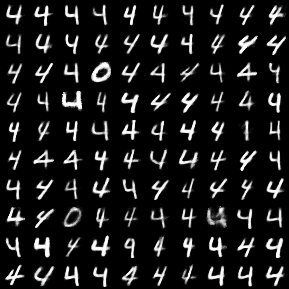
\includegraphics[width=\textwidth]{Images/l21R_8.png}
			\caption{Reconstruction}
		\end{subfigure}
		\hfill
		\begin{subfigure}[b]{0.3\textwidth}
			\centering
			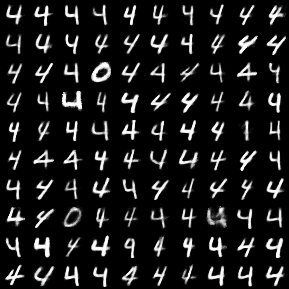
\includegraphics[width=\textwidth]{Images/l21L_8.png}
			\caption{Cleaned data}
		\end{subfigure}
		\hfill
		\begin{subfigure}[b]{0.3\textwidth}
			\centering
			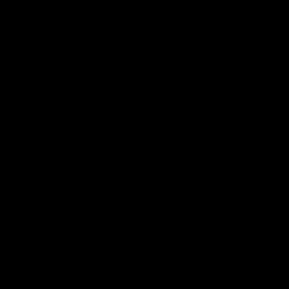
\includegraphics[width=\textwidth]{Images/l21S_8.png}
			\caption{Outliers detection}
		\end{subfigure}
		   \caption{Accuracy: $0.953$, precision: $1.00$, recall: $0.0386$, F1 score: $0.0743$}
   \end{figure}
\end{frame}

\begin{frame}
	\frametitle{$\lambda=4.0$}
	\begin{figure}
		\centering
		\begin{subfigure}[b]{0.3\textwidth}
			\centering
			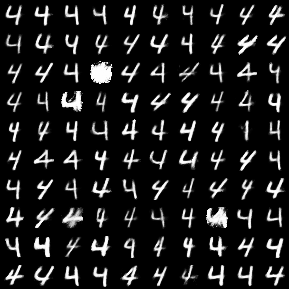
\includegraphics[width=\textwidth]{Images/l21R_4.png}
			\caption{Reconstruction}
		\end{subfigure}
		\hfill
		\begin{subfigure}[b]{0.3\textwidth}
			\centering
			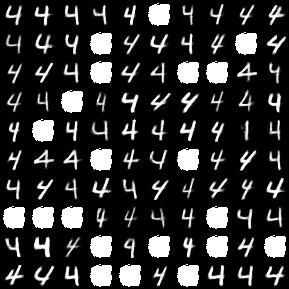
\includegraphics[width=\textwidth]{Images/l21L_4.png}
			\caption{Cleaned data}
		\end{subfigure}
		\hfill
		\begin{subfigure}[b]{0.3\textwidth}
			\centering
			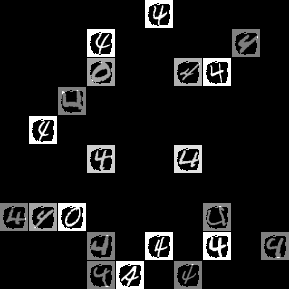
\includegraphics[width=\textwidth]{Images/l21S_4.png}
			\caption{Outliers detection}
		\end{subfigure}
		   \caption{Accuracy: $0.788$, precision: $0.167$, recall: $0.839$, F1 score: $0.278$}
   \end{figure}
\end{frame}

\begin{frame}
	\begin{itemize}
		\item The performance of the RDAE as outlied detector is compared with the one obtained using the isolation forest method.
		\item The isolation forest method was a SOTA method for outlied detection. It is based on the idea that outliers are few and different and are separated from the rest.
		\item These outliers gets recognized using isolation trees which try to separate points from others.
		\item The only parameter which is peculiar to the method and which gets selected with the same metrics is the outlier fraction (from $0$ to $0.5$)
	\end{itemize}
\end{frame}

\begin{frame}
	\frametitle{Isolation forest performance}
	\begin{figure}
		\centering
		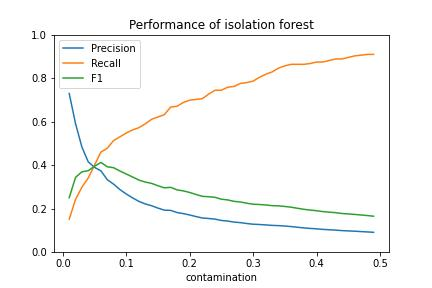
\includegraphics[width=0.8\linewidth]{Images/isolation_forest.jpg}
		\caption[]{Isolation forest performance}
	\end{figure}
\end{frame}

\begin{frame}
	\begin{itemize}
		\item The best isolation forest performance is $0.41$ with the outlier fraction set to the value of $0.06$ (which is really close to the outlier true fraction of $5\%$).
		\item This result is really close to the original article. The authors obtained a best $F_1$ score of $0.37$ with $0.11$ outlier fraction.
		\item The little difference is in my opinion related to the different datasets but they are comparable.
		\item In each case the performance by isolation forest is far worse than the RDAE.
	\end{itemize}
\end{frame}

\begin{frame}
	\frametitle{Time series experiment}
	\begin{itemize}
		\item I tried to apply this method to time series, on which we focused in this course.
		\item In this case we are going to use a dataset from the Numenta Anomaly Benchmark \hyperref{https://github.com/numenta/NAB/tree/master/data}{}{}{(NAB)}. The database is called machine temperature system failure.
		\item It is the sensor data of an internal component of a large, industrial mahcine. It should have $3$ anomalies: the first anomaly is a planned shutdown of the machine. The second anomaly is difficult to detect and directly led to the third anomaly, a catastrophic failure of the machine.
		\item Data has $22464$ timesteps in total. I chose to consider subsequences of length $144$. The final dataset has then $22321$ training time series.
		\item Data is normalized all togheter to be in $(0,1)$.
	\end{itemize}
\end{frame}

\begin{frame}
	\frametitle{RDAE architectures}
	I tried using two architectures for the autoencoder part in the RDAE.
	\begin{itemize}
		\item The first one is a Dense Neural Network with hidden layers of $60$ and $20$. It is trained for $20$ outer iterations and $50$ inner iterations for the autoencoder, a batch size of $256$ , $\epsilon=10^{-8}$.
		\item The second one is a LSTM with two layers of $32$ and $16$ units, $10$ outer iterations and $25$ inner iterations with same batch size as before. 
	\end{itemize}
\end{frame}

\begin{frame}
	\frametitle{Analysis}
	\begin{itemize}
		\item Since data is unlabeled we don't have a clear benchmark for finding the correct value for $\lambda$.
		\item I tried different values for $\lambda$ until the number of anomalies detected is nor too high nor too low.
		\item For each architecture I picked some random anomalies and non-anomalies, to show how the RDAE is acting on time series and to have a look at what kind of anomalies it detectes.
	\end{itemize}
\end{frame}

\begin{frame}
	\frametitle{Anomalies found}
	\begin{table}[width=\linewidth]
		\begin{tabular}{|c|c|c|c|c|c|c|c|c|c|}
		\hline
		\textbf{$\lambda$} & \textbf{$0.1$} & \textbf{$0.5$} & \textbf{$0.7$} & \textbf{$1.0$}  & \textbf{$2.0$} & \textbf{$3.0$} & \textbf{$3.2$} & \textbf{$3.3$} & \textbf{$4$}\\ \hline
		\textbf{Dense} & All       & $751$          & $250$          & $14$     & $0$            & $0$            & $0$            & $0$            & $0$ \\ \hline
		\textbf{LSTM}  & All        & $7525$         & $4208$         & $2068$  & $306$          & $109$          & $74$           & $9$            & $0$ \\ \hline
		\textbf{GRU}  & All        & $7277$         & $4505$         & $2454$  & $331$          & $139$          & $103$           & $80$            & $0$ \\ \hline
		\end{tabular}
		\caption[]{Anomalies found by the two architecures w.r.t. $\lambda$}
	\end{table}
\end{frame}

\begin{frame}
	\frametitle{Dense RDAE}
	\begin{figure}
		\centering
		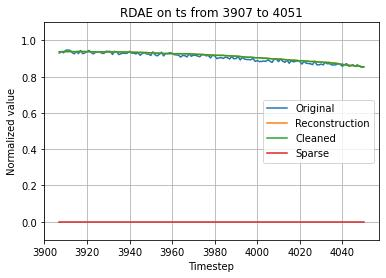
\includegraphics[width=0.7\linewidth]{Images/lam1.0ts_non_anomaly3907.jpg}
		\caption[]{Example of a non anomaly subsequence for $\lambda=1.0$}
	\end{figure}
\end{frame}

\begin{frame}
	\frametitle{Dense RDAE}
	\begin{figure}
		\centering
		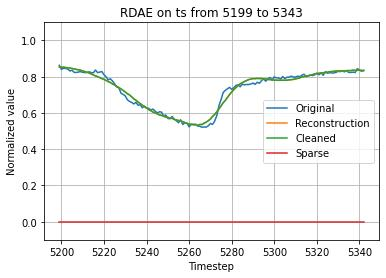
\includegraphics[width=0.7\linewidth]{Images/lam1.0ts_non_anomaly5199.jpg}
		\caption[]{Example of a non anomaly subsequence for $\lambda=1.0$}
	\end{figure}
\end{frame}

\begin{frame}
	\frametitle{Dense RDAE}
	\begin{figure}
		\centering
		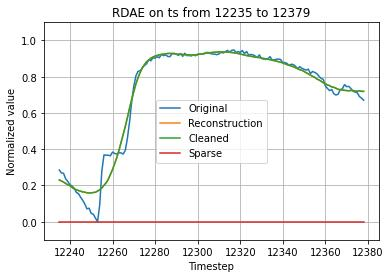
\includegraphics[width=0.7\linewidth]{Images/lam1.0ts_non_anomaly12235.jpg}
		\caption[]{Example of a non anomaly subsequence for $\lambda=1.0$}
	\end{figure}
\end{frame}

\begin{frame}
	\frametitle{Dense RDAE}
	\begin{figure}
		\centering
		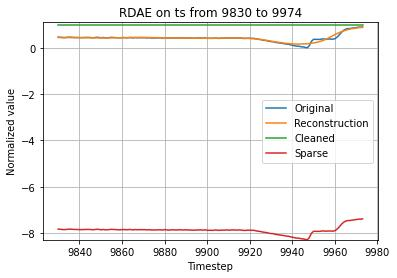
\includegraphics[width=0.7\linewidth]{Images/lam1.0ts_anomaly9830.jpg}
		\caption[]{Example of a anomaly subsequence for $\lambda=1.0$}
	\end{figure}
\end{frame}

\begin{frame}
	\frametitle{Dense RDAE}
	\begin{figure}
		\centering
		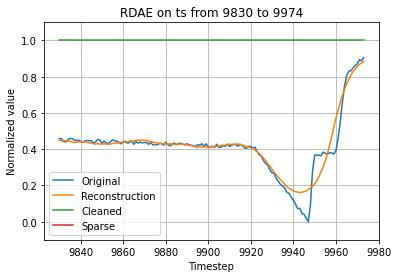
\includegraphics[width=0.7\linewidth]{Images/lam1.0ts_anomalyzoom9830.jpg}
		\caption[]{Example of a anomaly subsequence for $\lambda=1.0$}
	\end{figure}
\end{frame}

\begin{frame}
	\frametitle{Dense RDAE}
	\begin{figure}
		\centering
		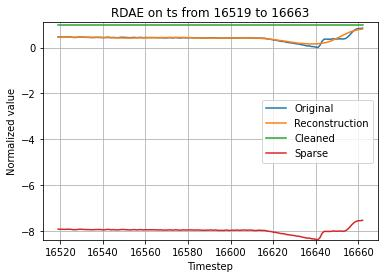
\includegraphics[width=0.7\linewidth]{Images/lam1.0ts_anomaly16519.jpg}
		\caption[]{Example of a anomaly subsequence for $\lambda=1.0$}
	\end{figure}
\end{frame}

\begin{frame}
	\frametitle{Dense RDAE}
	\begin{figure}
		\centering
		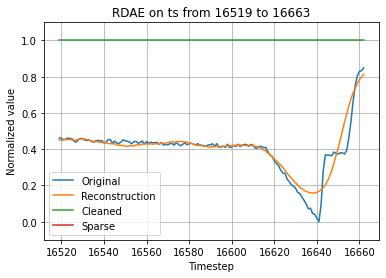
\includegraphics[width=0.7\linewidth]{Images/lam1.0ts_anomalyzoom16519.jpg}
		\caption[]{Example of a anomaly subsequence for $\lambda=1.0$}
	\end{figure}
\end{frame}

\begin{frame}
	\frametitle{Dense RDAE}
	\begin{figure}
		\centering
		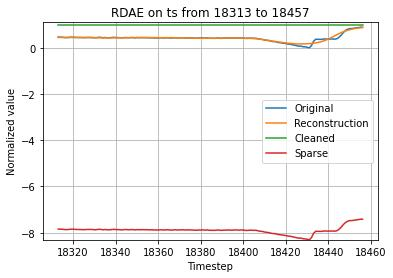
\includegraphics[width=0.7\linewidth]{Images/lam1.0ts_anomaly18313.jpg}
		\caption[]{Example of a anomaly subsequence for $\lambda=1.0$}
	\end{figure}
\end{frame}

\begin{frame}
	\frametitle{Dense RDAE}
	\begin{figure}
		\centering
		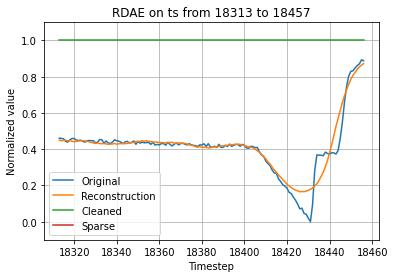
\includegraphics[width=0.7\linewidth]{Images/lam1.0ts_anomalyzoom18313.jpg}
		\caption[]{Example of a anomaly subsequence for $\lambda=1.0$}
	\end{figure}
\end{frame}

\begin{frame}
	\frametitle{Dense RDAE}
	\begin{itemize}
		\item All of the anomalies found reach the $0$ value (min temperature of all time series).
		\item Note that the different anomalies found DO NOT overlap. So each of the failures is only recognized once.
		\item This may also create problems, since as you can see one failure is not recognized as anomaly.
		\item In general, the reconstruction is a non-noisy version of the signal.
	\end{itemize}
\end{frame}

\begin{frame}
	\frametitle{LSTM RDAE}
	\begin{figure}
		\centering
		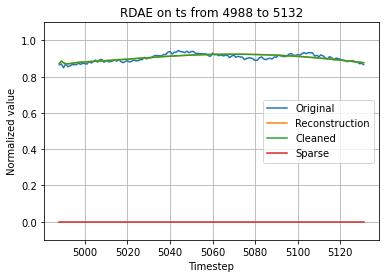
\includegraphics[width=0.7\linewidth]{Images/LSTMlam3.3ts_non_anomaly4988.jpg}
		\caption[]{Example of a non anomaly subsequence for $\lambda=3.3$}
	\end{figure}
\end{frame}

\begin{frame}
	\frametitle{LSTM RDAE}
	\begin{figure}
		\centering
		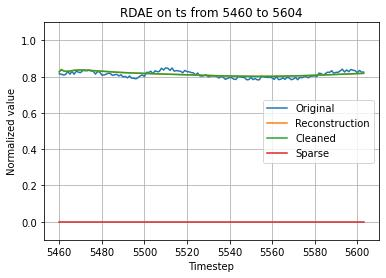
\includegraphics[width=0.7\linewidth]{Images/LSTMlam3.3ts_non_anomaly5460.jpg}
		\caption[]{Example of a non anomaly subsequence for $\lambda=3.3$}
	\end{figure}
\end{frame}

\begin{frame}
	\frametitle{LSTM RDAE}
	\begin{figure}
		\centering
		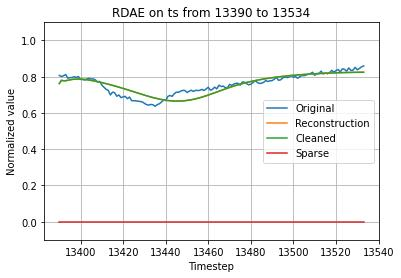
\includegraphics[width=0.7\linewidth]{Images/LSTMlam3.3ts_non_anomaly13390.jpg}
		\caption[]{Example of a non anomaly subsequence for $\lambda=3.3$}
	\end{figure}
\end{frame}

\begin{frame}
	\frametitle{LSTM RDAE}
	\begin{figure}
		\centering
		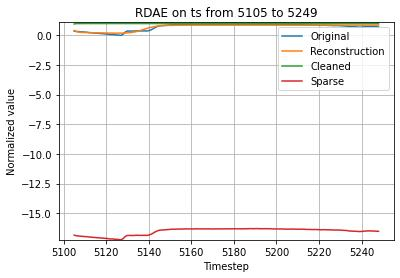
\includegraphics[width=0.7\linewidth]{Images/LSTMlam3.3ts_anomaly5105.jpg}
		\caption[]{Example of a anomaly subsequence for $\lambda=3.3$}
	\end{figure}
\end{frame}

\begin{frame}
	\frametitle{LSTM RDAE}
	\begin{figure}
		\centering
		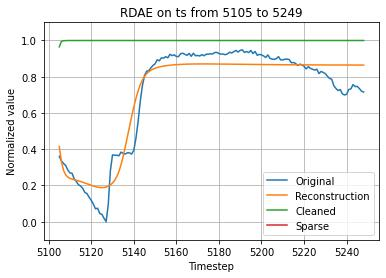
\includegraphics[width=0.7\linewidth]{Images/LSTMlam3.3ts_anomalyzoom5105.jpg}
		\caption[]{Example of a anomaly subsequence for $\lambda=3.3$}
	\end{figure}
\end{frame}

\begin{frame}
	\frametitle{LSTM RDAE}
	\begin{figure}
		\centering
		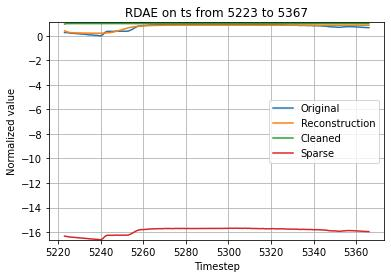
\includegraphics[width=0.7\linewidth]{Images/LSTMlam3.3ts_anomaly5223.jpg}
		\caption[]{Example of a anomaly subsequence for $\lambda=3.3$}
	\end{figure}
\end{frame}

\begin{frame}
	\frametitle{LSTM RDAE}
	\begin{figure}
		\centering
		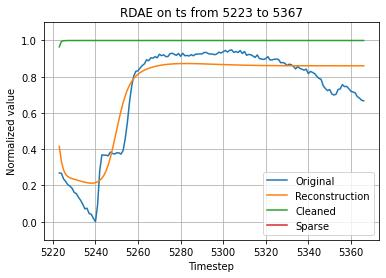
\includegraphics[width=0.7\linewidth]{Images/LSTMlam3.3ts_anomalyzoom5223.jpg}
		\caption[]{Example of a anomaly subsequence for $\lambda=3.3$}
	\end{figure}
\end{frame}

\begin{frame}
	\frametitle{LSTM RDAE}
	\begin{figure}
		\centering
		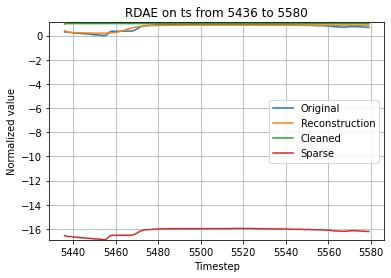
\includegraphics[width=0.7\linewidth]{Images/LSTMlam3.3ts_anomaly5436.jpg}
		\caption[]{Example of a anomaly subsequence for $\lambda=3.3$}
	\end{figure}
\end{frame}

\begin{frame}
	\frametitle{LSTM RDAE}
	\begin{figure}
		\centering
		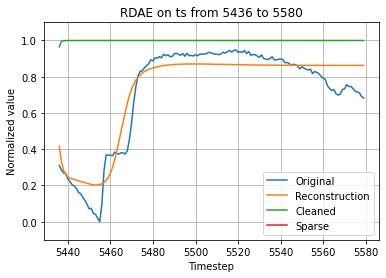
\includegraphics[width=0.7\linewidth]{Images/LSTMlam3.3ts_anomalyzoom5436.jpg}
		\caption[]{Example of a anomaly subsequence for $\lambda=3.3$}
	\end{figure}
\end{frame}

\begin{frame}
	\frametitle{LSTM RDAE}
	\begin{itemize}
		\item All of the anomalies found reach the $0$ value (min temperature of all time series).
		\item Also in this case different anomalies found DO NOT overlap. So each of the failures is only recognized once. In this case this happens at the beginning of the subsequence
		\item The reconstruction here is far worse than in the dense case.
		\item Performance could be improved using more parameters in the LSTM case. Note that computation time is much higher ($\sim 4$ minutes for dense, $\sim 20$ minutes for LSTM, with the help of a RTX3070 laptop).
	\end{itemize}
\end{frame}

\begin{frame}
	\frametitle{GRU RDAE}
	\begin{figure}
		\centering
		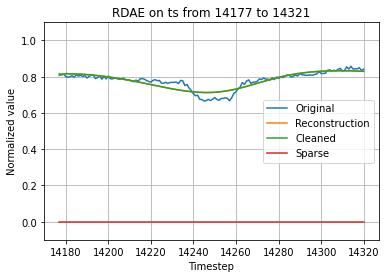
\includegraphics[width=0.7\linewidth]{Images/GRUlam3.3ts_non_anomalyzoom14177.jpg}
		\caption[]{Example of a non anomaly subsequence for $\lambda=3.3$}
	\end{figure}
\end{frame}

\begin{frame}
	\frametitle{GRU RDAE}
	\begin{figure}
		\centering
		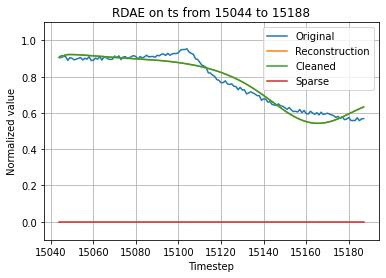
\includegraphics[width=0.7\linewidth]{Images/GRUlam3.3ts_non_anomalyzoom15044.jpg}
		\caption[]{Example of a non anomaly subsequence for $\lambda=3.3$}
	\end{figure}
\end{frame}

\begin{frame}
	\frametitle{GRU RDAE}
	\begin{figure}
		\centering
		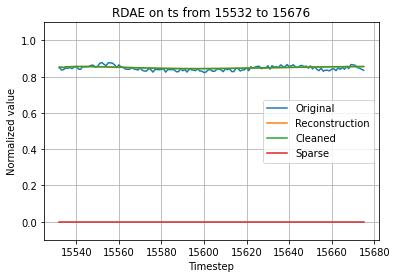
\includegraphics[width=0.7\linewidth]{Images/GRUlam3.3ts_non_anomalyzoom15532.jpg}
		\caption[]{Example of a non anomaly subsequence for $\lambda=3.3$}
	\end{figure}
\end{frame}

\begin{frame}
	\frametitle{GRU RDAE}
	\begin{figure}
		\centering
		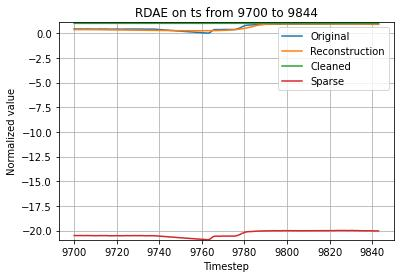
\includegraphics[width=0.7\linewidth]{Images/GRUlam3.3ts_anomaly9700.jpg}
		\caption[]{Example of a anomaly subsequence for $\lambda=3.3$}
	\end{figure}
\end{frame}

\begin{frame}
	\frametitle{GRU RDAE}
	\begin{figure}
		\centering
		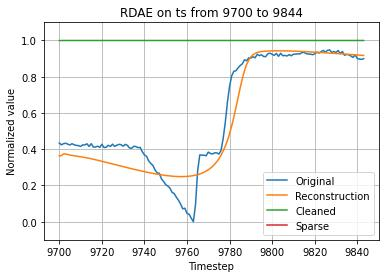
\includegraphics[width=0.7\linewidth]{Images/GRUlam3.3ts_anomalyzoom9700.jpg}
		\caption[]{Example of a anomaly subsequence for $\lambda=3.3$}
	\end{figure}
\end{frame}

\begin{frame}
	\frametitle{GRU RDAE}
	\begin{figure}
		\centering
		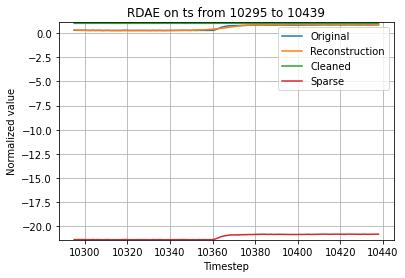
\includegraphics[width=0.7\linewidth]{Images/GRUlam3.3ts_anomaly10295.jpg}
		\caption[]{Example of a anomaly subsequence for $\lambda=3.3$}
	\end{figure}
\end{frame}

\begin{frame}
	\frametitle{GRU RDAE}
	\begin{figure}
		\centering
		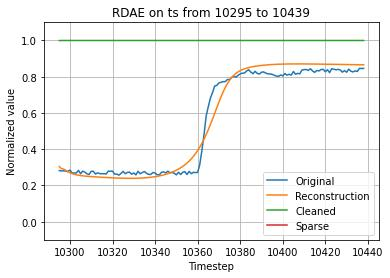
\includegraphics[width=0.7\linewidth]{Images/GRUlam3.3ts_anomalyzoom10295.jpg}
		\caption[]{Example of a anomaly subsequence for $\lambda=3.3$}
	\end{figure}
\end{frame}

\begin{frame}
	\frametitle{GRU RDAE}
	\begin{figure}
		\centering
		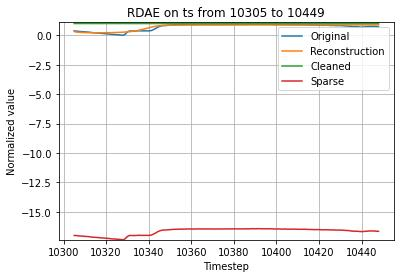
\includegraphics[width=0.7\linewidth]{Images/GRUlam3.3ts_anomaly10305.jpg}
		\caption[]{Example of a anomaly subsequence for $\lambda=3.3$}
	\end{figure}
\end{frame}

\begin{frame}
	\frametitle{GRU RDAE}
	\begin{figure}
		\centering
		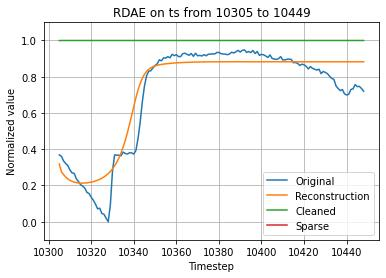
\includegraphics[width=0.7\linewidth]{Images/GRUlam3.3ts_anomalyzoom10305.jpg}
		\caption[]{Example of a anomaly subsequence for $\lambda=3.3$}
	\end{figure}
\end{frame}

\begin{frame}
	\frametitle{GRU RDAE}
	\begin{itemize}
		\item In this case, not all of the anomalies found reach the $0$ value.
		\item Also in this case different anomalies found DO NOT overlap. So each of the failures is only recognized once. With GRU this happens in different parts of the subsequence.
		\item Also here the reconstruction is far worse than in the dense case.
		\item Again we could increase parameters for better performance. Computation here required $\sim 12$ minutes with GPU.
	\end{itemize}
\end{frame}

\begin{frame}
\centering{\hyperref{https://github.com/AlexThirty/SaMLMfTSA}{}{}{https://github.com/AlexThirty/SaMLMfTSA}}
	\Huge{\centerline{Thank you!}} 
\end{frame}

\nocite{RAE}
\nocite{DATA}
\nocite{RPCA}
\nocite{PROX}

\bibliographystyle{alpha}
\bibliography{Bibliography}



%----------------------------------------------------------------------------------------

\end{document}
